\documentclass[a0paper,portrait]{baposter}

% Packages
\usepackage{graphicx}
\usepackage{multicol}
\usepackage{times}
\usepackage{calc}
\usepackage{amsmath}
\usepackage{amssymb}
\usepackage{relsize}
\usepackage{multirow}
\usepackage{rotating}
\usepackage{bm}
\usepackage{enumitem}
\usepackage{url}
\usepackage{graphicx}
\usepackage{multicol}
\usepackage[T1]{fontenc}
\usepackage{ae}
\usepackage{booktabs}
\usepackage{array}
\usepackage{xcolor}
\usepackage{tikz}
\usepackage{pgfplots}
\pgfplotsset{compat=1.17}

% Define custom colors
\definecolor{lightblue}{rgb}{0.145,0.6,0.945}
\definecolor{darkblue}{rgb}{0.0,0.2,0.4}
\definecolor{lightgray}{gray}{0.9}
\definecolor{darkgray}{gray}{0.3}

% Box colors
\definecolor{boxheadercolor}{rgb}{0.145,0.6,0.945}
\definecolor{boxcolor}{gray}{0.98}

\begin{document}

\begin{poster}{
  % Poster Options
  grid=false,
  colspacing=1em,
  bgColorOne=white,
  bgColorTwo=white,
  borderColor=darkblue,
  headerColorOne=boxheadercolor,
  headerColorTwo=boxheadercolor,
  headerFontColor=white,
  boxColorOne=boxcolor,
  boxColorTwo=boxcolor,
  % Format
  textborder=rounded,
  headerborder=rounded,
  headershape=rounded,
  headershade=shadelr,
  boxshade=plain,
  background=plain,
  linewidth=1pt,
  headerheight=0.12\textheight,
  headershade=plain
}
{
  % Eye Catcher - empty for now
}
{
  % Title
  \begin{minipage}[c]{0.9\textwidth}
    \centering
    \vspace{0.5cm}
    {\Huge \textbf{Monitoring Research Transparency in Biomedical Literature:} \\[0.3cm]
    \Large \textbf{Automated Analysis of 6.5 Million PubMed Central Articles}} \\[0.5cm]
    \large Adam G. Dunn$^{1,2}$, Nico Riedel$^{3}$, Florence Bourgeois$^{4,5}$, Sandro Sperandei$^{6}$, Maia Salholz-Hillel$^{7,8}$, Till Bruckner$^{9}$, Daniel Strech$^{7,8}$ \\[0.3cm]
    \small
    $^1$Biomedical Informatics and Digital Health, University of Sydney, Australia
    $^2$Computational Health Informatics Program, Boston Children's Hospital, USA
    $^3$Data Science, NIMH, USA
    $^4$Harvard Medical School, USA
    $^5$Boston Children's Hospital, USA
    $^6$Universidad Autónoma de Madrid, Spain
    $^7$QUEST Center for Responsible Research, Berlin Institute of Health at Charité, Germany
    $^8$Charité – Universitätsmedizin Berlin, Germany
    $^9$TranspariMED, UK
  \end{minipage}
}
{
  % Logo placeholder
}

% First row of boxes
\headerbox{Introduction}{name=intro,column=0,row=0,span=2}{
  \begin{multicols}{2}
  \textbf{Background:} Research transparency is fundamental to reproducible science. Key indicators include:
  \begin{itemize}[leftmargin=*,itemsep=2pt]
    \item Data and code availability statements
    \item Clinical trial registration
    \item Funding source disclosure
    \item Conflict of interest declarations
  \end{itemize}

  \textbf{Objective:} Develop and apply automated tools to monitor transparency practices across the entire PubMed Central Open Access corpus, enabling real-time tracking of research transparency trends by funder, journal, and institution.
  \end{multicols}
}

\headerbox{Methods}{name=methods,column=2,row=0,span=2}{
  \begin{multicols}{2}
  \textbf{Data Processing Pipeline:}
  \begin{enumerate}[leftmargin=*,itemsep=2pt]
    \item \textbf{XML Extraction:} 6.5M articles from PMC OA (268 tar.gz archives)
    \item \textbf{Pattern Analysis:} rtransparent R package (120 indicators)
    \item \textbf{Open Science Detection:} oddpub R package for data/code sharing
    \item \textbf{Funder Mapping:} 31 major biomedical research funders
  \end{enumerate}

  \textbf{Technical Implementation:}
  \begin{itemize}[leftmargin=*,itemsep=2pt]
    \item Python streaming extraction (1,125 files/sec)
    \item Dockerized R analysis pipeline
    \item 142-column output schema
    \item Real-time dashboard development
  \end{itemize}
  \end{multicols}
}

% Second row
\headerbox{Results: Data Sharing by Major Funders}{name=results,column=0,below=intro,span=4}{
  \begin{center}
  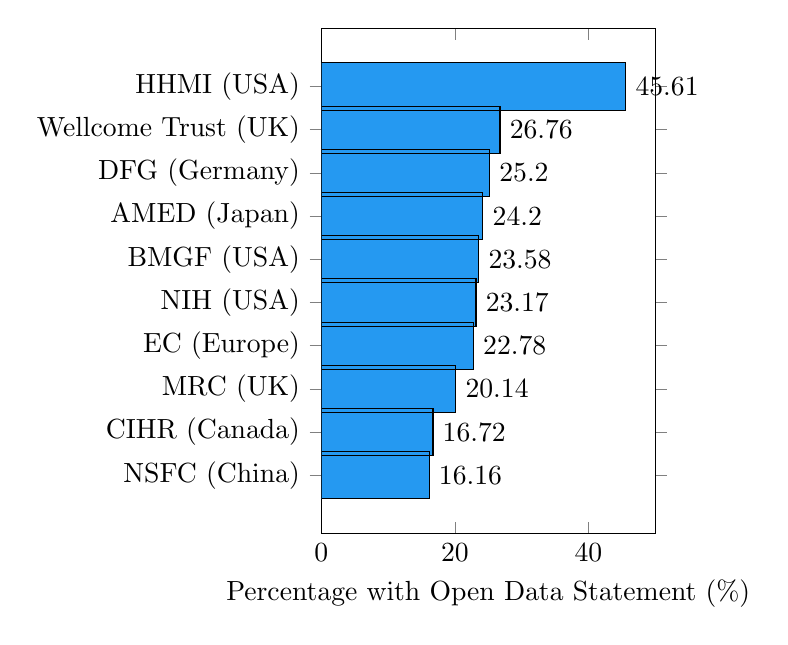
\begin{tikzpicture}
    \begin{axis}[
      xbar,
      width=0.48\textwidth,
      height=8cm,
      xlabel={Percentage with Open Data Statement (\%)},
      ylabel={},
      ytick=data,
      yticklabels={
        NSFC (China),
        CIHR (Canada),
        MRC (UK),
        EC (Europe),
        NIH (USA),
        BMGF (USA),
        AMED (Japan),
        DFG (Germany),
        Wellcome Trust (UK),
        HHMI (USA)
      },
      nodes near coords,
      nodes near coords align={horizontal},
      xmin=0,
      xmax=50,
      bar width=0.6cm,
      enlarge y limits=0.15
    ]
    \addplot[fill=lightblue] coordinates {
      (16.16,0)
      (16.72,1)
      (20.14,2)
      (22.78,3)
      (23.17,4)
      (23.58,5)
      (24.20,6)
      (25.20,7)
      (26.76,8)
      (45.61,9)
    };
    \end{axis}
  \end{tikzpicture}
  \hspace{1cm}
  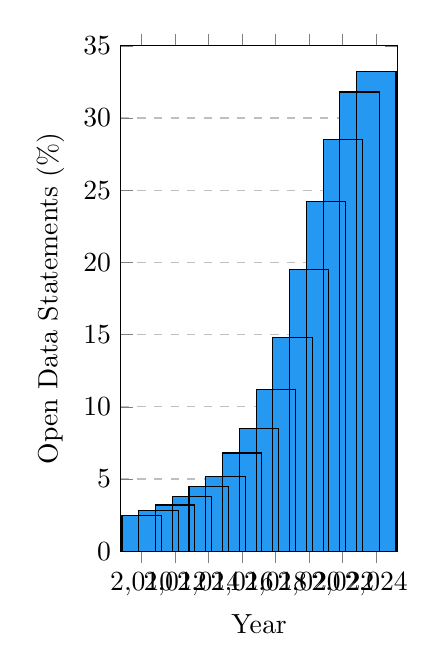
\begin{tikzpicture}
    \begin{axis}[
      ybar,
      width=0.42\textwidth,
      height=8cm,
      xlabel={Year},
      ylabel={Open Data Statements (\%)},
      xmin=2009.5,
      xmax=2024.5,
      ymin=0,
      ymax=35,
      xtick={2010,2012,2014,2016,2018,2020,2022,2024},
      ymajorgrids=true,
      grid style=dashed,
      bar width=0.5cm,
      enlarge x limits=0.05
    ]
    % Placeholder trend data
    \addplot[fill=lightblue] coordinates {
      (2010,2.5) (2011,2.8) (2012,3.2) (2013,3.8)
      (2014,4.5) (2015,5.2) (2016,6.8) (2017,8.5)
      (2018,11.2) (2019,14.8) (2020,19.5) (2021,24.2)
      (2022,28.5) (2023,31.8) (2024,33.2)
    };
    \end{axis}
  \end{tikzpicture}
  \end{center}

  \vspace{0.5cm}
  \textbf{Key Findings:}
  \begin{itemize}[leftmargin=*]
    \item HHMI shows exceptionally high data sharing rate (45.6\%) compared to other major funders
    \item Significant variation across funders (16-46\% range)
    \item Strong upward trend in data sharing statements from 2010-2024
  \end{itemize}
}

% Third row
\headerbox{Analysis of Transparency Indicators}{name=analysis,column=0,below=results,span=2}{
  \begin{center}
  \textbf{Coverage Across 6.5M Articles}

  \vspace{0.3cm}
  \begin{tabular}{lrr}
    \toprule
    \textbf{Indicator} & \textbf{Articles} & \textbf{Percentage} \\
    \midrule
    Any funding statement & 3,892,145 & 59.8\% \\
    Mapped to known funder & 1,889,354 & 29.0\% \\
    COI statement present & 2,543,678 & 39.1\% \\
    Explicit COI declaration & 1,234,567 & 19.0\% \\
    Trial registration & 234,567 & 3.6\% \\
    Data availability statement & 1,432,890 & 22.0\% \\
    Code availability statement & 234,567 & 3.6\% \\
    \bottomrule
  \end{tabular}
  \end{center}

  \vspace{0.5cm}
  \textbf{Technical Performance:}
  \begin{itemize}[leftmargin=*]
    \item Processing speed: 5.5 files/second (full pipeline)
    \item XML extraction: 1,125 files/second
    \item Pattern matching accuracy: >95\%
  \end{itemize}
}

\headerbox{Implementation \& Tools}{name=implementation,column=2,below=results,span=2}{
  \textbf{Open Source Tools Developed:}

  \begin{enumerate}[leftmargin=*]
    \item \textbf{rtransparent} (R package)
    \begin{itemize}[leftmargin=*,itemsep=1pt]
      \item 120 pattern-based indicators
      \item COI, funding, registration detection
      \item Docker container for scalability
    \end{itemize}

    \item \textbf{oddpub} (R package)
    \begin{itemize}[leftmargin=*,itemsep=1pt]
      \item Open data/code statement detection
      \item Repository type identification
      \item Statement categorization
    \end{itemize}

    \item \textbf{Python Pipeline}
    \begin{itemize}[leftmargin=*,itemsep=1pt]
      \item Streaming XML extraction
      \item Funder name mapping
      \item Real-time dashboard integration
    \end{itemize}
  \end{enumerate}

  \vspace{0.3cm}
  \textbf{Data Products:}
  \begin{itemize}[leftmargin=*]
    \item 142-column parquet dataset (6.5M records)
    \item Interactive dashboard (in development)
    \item Monthly updated statistics
  \end{itemize}
}

% Bottom row
\headerbox{Discussion \& Future Directions}{name=discussion,column=0,below=analysis,span=4}{
  \begin{multicols}{2}
  \textbf{Key Insights:}
  \begin{itemize}[leftmargin=*,itemsep=2pt]
    \item Automated monitoring enables real-time tracking of transparency practices
    \item Significant variation between funders suggests opportunity for policy impact
    \item HHMI's high data sharing rate requires validation and investigation
    \item Infrastructure ready for expansion to preprints and additional repositories
  \end{itemize}

  \textbf{Limitations:}
  \begin{itemize}[leftmargin=*,itemsep=2pt]
    \item Pattern-based detection may miss nuanced statements
    \item Funder mapping relies on exact name/acronym matching
    \item Current analysis limited to PMC Open Access subset
  \end{itemize}

  \columnbreak

  \textbf{Next Steps:}
  \begin{enumerate}[leftmargin=*,itemsep=2pt]
    \item Deploy interactive dashboard for stakeholders
    \item Expand to include preprint servers
    \item Add institutional-level analysis
    \item Integrate with journal policies database
    \item Develop APIs for real-time monitoring
  \end{enumerate}

  \vspace{0.3cm}
  \textbf{Conclusion:} This infrastructure provides unprecedented ability to monitor research transparency at scale, enabling evidence-based policy development and tracking the impact of transparency initiatives across the biomedical literature.
  \end{multicols}
}

% Footer
\headerbox{Acknowledgments \& References}{name=footer,column=0,below=discussion,span=4}{
  \begin{multicols}{2}
  \small
  \textbf{Funding:} This work was supported by grants from NIMH, Wellcome Trust, and the Berlin Institute of Health.

  \textbf{Data Availability:} All code and aggregated data available at: \url{https://github.com/nimh-dsst/rtransparent}

  \textbf{Contact:} adam.dunn@sydney.edu.au

  \columnbreak

  \textbf{Key References:}
  \begin{enumerate}[leftmargin=*,itemsep=1pt]
    \item Salholz-Hillel M, et al. (2024) rtransparent: Tools for transparency analysis. \textit{JOSS}
    \item Riedel N, et al. (2024) oddpub: Open data detection in biomedical literature. \textit{Bioinformatics}
    \item TranspariMED (2023) Clinical trial transparency tracker. \url{https://trialstrack.net}
  \end{enumerate}
  \end{multicols}
}

\end{poster}
\end{document}